% Options for packages loaded elsewhere
\PassOptionsToPackage{unicode}{hyperref}
\PassOptionsToPackage{hyphens}{url}
%
\documentclass[
  ignorenonframetext,
]{beamer}
\usepackage{pgfpages}
\setbeamertemplate{caption}[numbered]
\setbeamertemplate{caption label separator}{: }
\setbeamercolor{caption name}{fg=normal text.fg}
\beamertemplatenavigationsymbolsempty
% Prevent slide breaks in the middle of a paragraph
\widowpenalties 1 10000
\raggedbottom
\setbeamertemplate{part page}{
  \centering
  \begin{beamercolorbox}[sep=16pt,center]{part title}
    \usebeamerfont{part title}\insertpart\par
  \end{beamercolorbox}
}
\setbeamertemplate{section page}{
  \centering
  \begin{beamercolorbox}[sep=12pt,center]{part title}
    \usebeamerfont{section title}\insertsection\par
  \end{beamercolorbox}
}
\setbeamertemplate{subsection page}{
  \centering
  \begin{beamercolorbox}[sep=8pt,center]{part title}
    \usebeamerfont{subsection title}\insertsubsection\par
  \end{beamercolorbox}
}
\AtBeginPart{
  \frame{\partpage}
}
\AtBeginSection{
  \ifbibliography
  \else
    \frame{\sectionpage}
  \fi
}
\AtBeginSubsection{
  \frame{\subsectionpage}
}
\usepackage{amsmath,amssymb}
\usepackage{lmodern}
\usepackage{ifxetex,ifluatex}
\ifnum 0\ifxetex 1\fi\ifluatex 1\fi=0 % if pdftex
  \usepackage[T1]{fontenc}
  \usepackage[utf8]{inputenc}
  \usepackage{textcomp} % provide euro and other symbols
\else % if luatex or xetex
  \usepackage{unicode-math}
  \defaultfontfeatures{Scale=MatchLowercase}
  \defaultfontfeatures[\rmfamily]{Ligatures=TeX,Scale=1}
\fi
\usecolortheme{dolphin}
% Use upquote if available, for straight quotes in verbatim environments
\IfFileExists{upquote.sty}{\usepackage{upquote}}{}
\IfFileExists{microtype.sty}{% use microtype if available
  \usepackage[]{microtype}
  \UseMicrotypeSet[protrusion]{basicmath} % disable protrusion for tt fonts
}{}
\makeatletter
\@ifundefined{KOMAClassName}{% if non-KOMA class
  \IfFileExists{parskip.sty}{%
    \usepackage{parskip}
  }{% else
    \setlength{\parindent}{0pt}
    \setlength{\parskip}{6pt plus 2pt minus 1pt}}
}{% if KOMA class
  \KOMAoptions{parskip=half}}
\makeatother
\usepackage{xcolor}
\IfFileExists{xurl.sty}{\usepackage{xurl}}{} % add URL line breaks if available
\IfFileExists{bookmark.sty}{\usepackage{bookmark}}{\usepackage{hyperref}}
\hypersetup{
  hidelinks,
  pdfcreator={LaTeX via pandoc}}
\urlstyle{same} % disable monospaced font for URLs
\newif\ifbibliography
\usepackage{graphicx}
\makeatletter
\def\maxwidth{\ifdim\Gin@nat@width>\linewidth\linewidth\else\Gin@nat@width\fi}
\def\maxheight{\ifdim\Gin@nat@height>\textheight\textheight\else\Gin@nat@height\fi}
\makeatother
% Scale images if necessary, so that they will not overflow the page
% margins by default, and it is still possible to overwrite the defaults
% using explicit options in \includegraphics[width, height, ...]{}
\setkeys{Gin}{width=\maxwidth,height=\maxheight,keepaspectratio}
% Set default figure placement to htbp
\makeatletter
\def\fps@figure{htbp}
\makeatother
\setlength{\emergencystretch}{3em} % prevent overfull lines
\providecommand{\tightlist}{%
  \setlength{\itemsep}{0pt}\setlength{\parskip}{0pt}}
\setcounter{secnumdepth}{-\maxdimen} % remove section numbering
\usepackage{caption}
\captionsetup[figure]{labelformat=empty}
\ifluatex
  \usepackage{selnolig}  % disable illegal ligatures
\fi

\title{P8158 - Must Athletes be Tough?\\
Effects of Athletic Identity and Resilience on Well-Being during
COVID-19}
\author{Waveley Qiu, Yihan Qiu, Yuanyuan Zeng}
\date{2022-05-04}

\begin{document}
\frame{\titlepage}

\begin{frame}{Motivation}
\protect\hypertarget{motivation}{}
\begin{itemize}
\item
  The onset of COVID-19 affected almost every sphere of work and
  leisure.
\item
  We are interested in investigating the impact athletic identity may
  have on athletes' overall well-being, particularly as the context of a
  global pandemic may have dramatically impacted one's experience of
  playing a sport/being an athlete.
\end{itemize}
\end{frame}

\begin{frame}{Resilience, Healthy Lifestyle, and Mental Health}
\protect\hypertarget{resilience-healthy-lifestyle-and-mental-health}{}
\begin{itemize}
\item
  Resilience and healthy lifestyle are both characteristics that are
  associated with improved mental health.
\item
  We hypothesize that the effect that being a devoted athlete has on
  overall well-being would be mediated through these two
  characteristics, and will endeavor to investigate the relationships
  between these variables as well.
\end{itemize}
\end{frame}

\begin{frame}{Methodology}
\protect\hypertarget{methodology}{}
\begin{enumerate}
\tightlist
\item
  Conduct EFA and CFA to determine which observed variables underlie our
  latent variables of interest.
\item
  Evaluate reliability of the determined latent structures with
  Chronbach's alpha.
\item
  Construct SEM(s) to quantify the relationship between our constructed
  latent variables and mental health score.
\end{enumerate}
\end{frame}

\begin{frame}{Data: Athlete Mental Health Survey}
\protect\hypertarget{data-athlete-mental-health-survey}{}
The dataset we selected contains responses for several surveys
administered in the UK to assess athlete (and non-athlete) mental health
and well-being after the country's first COVID-19 lockdown.

These surveys include:

\begin{itemize}
\item
  Athletic Identity Scale (AIMS)
\item
  The Brief Resilience Scale
\item
  Mental Health Continuum Short Form (MHC-SF)
\end{itemize}

In total, 753 individuals were interviewed -- we will focus our analysis
on the 363 athletes represented in this study.
\end{frame}

\begin{frame}{Latent Variable 1: Athletic Identity}
\protect\hypertarget{latent-variable-1-athletic-identity}{}
\begin{figure}
\centering
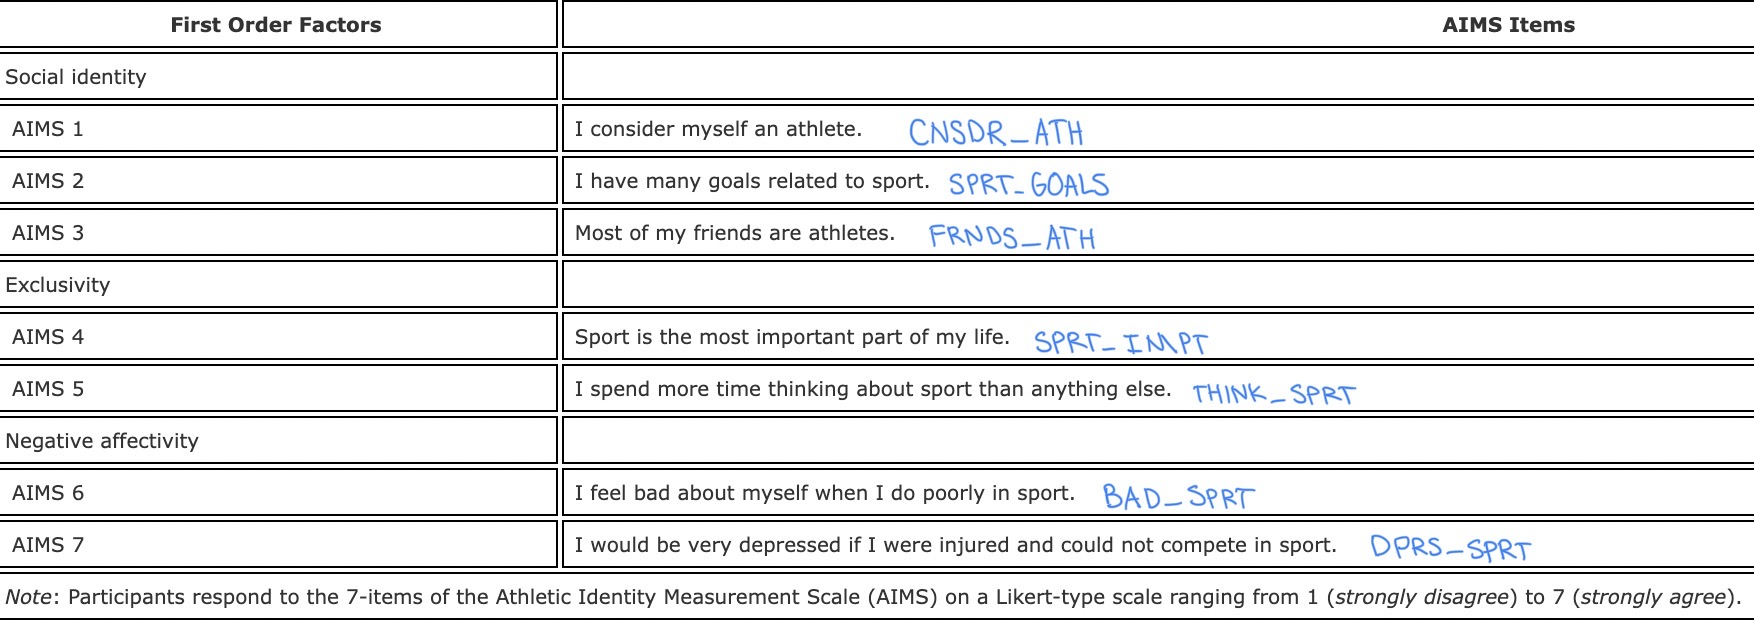
\includegraphics{images/aims_annotated.jpg}
\caption{Athletic Identity Scale (AIMS)}
\end{figure}
\end{frame}

\begin{frame}[fragile]{Latent Variable 1 (Athletic Identity): EFA}
\protect\hypertarget{latent-variable-1-athletic-identity-efa}{}
After conducting EFA, we first propose that there are three latent
variables underlying the AIMS variables, structured as follows:

\begin{itemize}
\tightlist
\item
  \texttt{external\_identity} (comprised of \texttt{sprt\_goals},
  \texttt{cnsdr\_ath}, \texttt{frnds\_ath})
\item
  \texttt{internal\_value} (comprised of \texttt{sprt\_impt},
  \texttt{think\_sprt})
\item
  \texttt{negative\_events} (comprised of \texttt{dprs\_sprt},
  \texttt{bad\_sprt})
\end{itemize}
\end{frame}

\begin{frame}[fragile]{Latent Variable 1 (Athletic Identity):
Reliability}
\protect\hypertarget{latent-variable-1-athletic-identity-reliability}{}
Chronbach's alpha were reasonable for \texttt{internal\_value} and
\texttt{negative\_events} (0.81 and 0.63, respectively), with no
variables indicated that could be dropped to improve reliability.

However, for \texttt{external\_identity}:

\centering

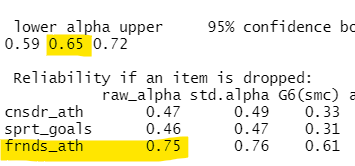
\includegraphics{images/athletic_identity_alpha.png}

Since Chronbach's alpha for \texttt{external\_identity} would improve
significantly if \texttt{frnds\_ath} is removed, we decided to remove
this variable from the latent structure.
\end{frame}

\begin{frame}[fragile]{Latent Variable 1 (Athletic Identity): CFA}
\protect\hypertarget{latent-variable-1-athletic-identity-cfa}{}
We hypothesized that there exists a second-order latent variable,
\texttt{athletic\_identity}, underlying the latent variables
\texttt{external\_identity}, \texttt{internal\_value}, and
\texttt{negative\_events}. Conducting a CFA allows us to evaluate this
hypothesis:

\centering

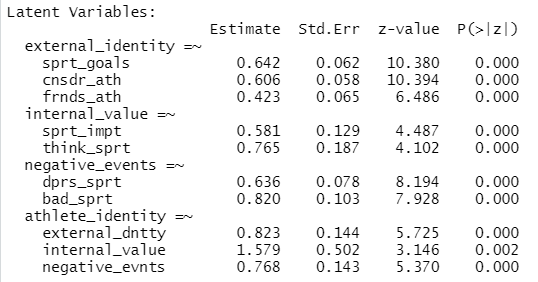
\includegraphics{images/athletic_identity_cfa.png}

Fit statistics: CFI \textgreater{} 0.99, RMSEA \textless{} 0.05,
\(\chi^2\) = 0.514
\end{frame}

\begin{frame}{Latent Variable 2: Resilience}
\protect\hypertarget{latent-variable-2-resilience}{}
\centering

\begin{figure}
\centering
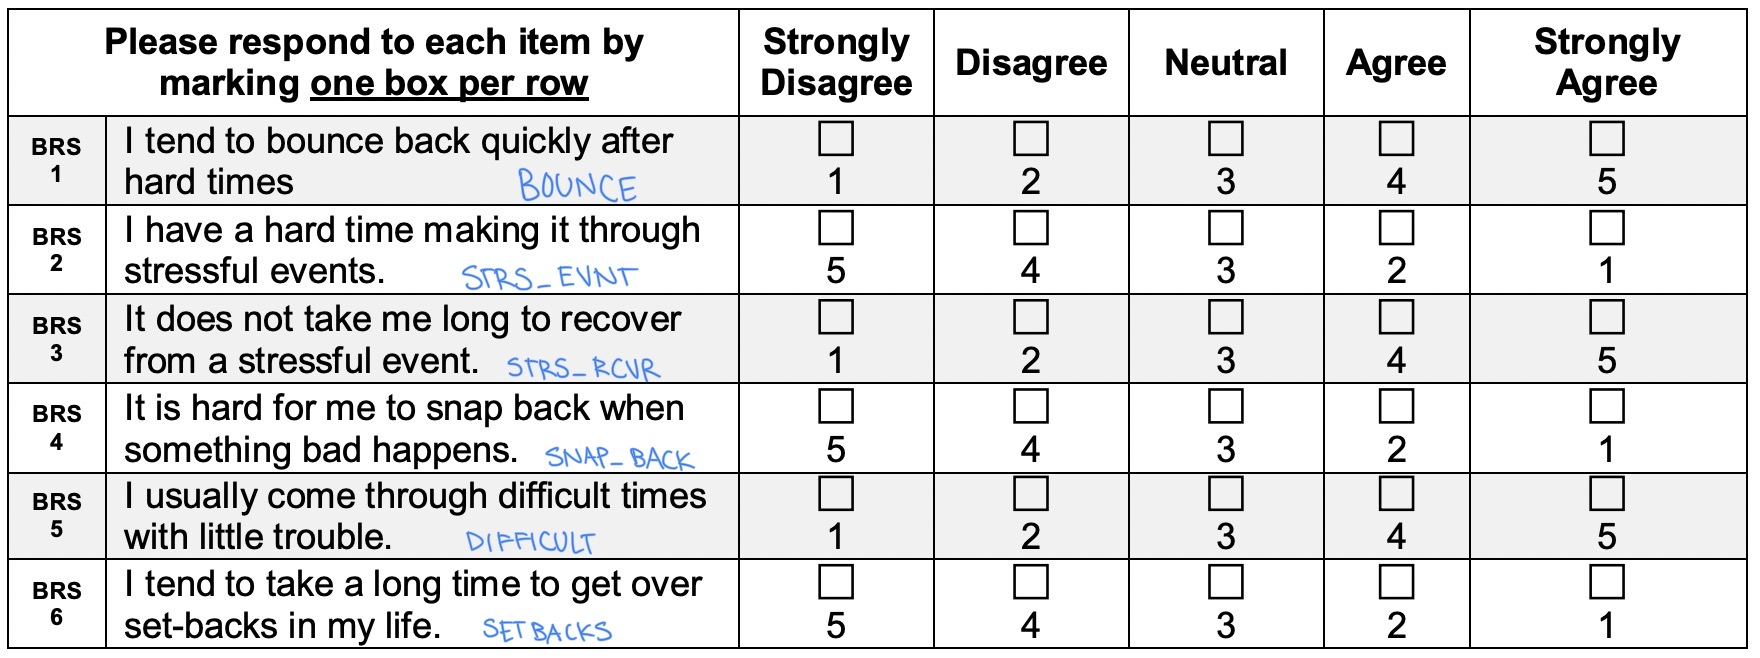
\includegraphics{images/resilience_annotated.jpg}
\caption{The Brief Resilience Scale (BRS)}
\end{figure}
\end{frame}

\begin{frame}{Latent Variable 2 (Resilience): EFA}
\protect\hypertarget{latent-variable-2-resilience-efa}{}
After running EFA on 1- and 2- factor models, we find that the 1-factor
model, containing all variables from the scale fits the best.
\end{frame}

\begin{frame}{Latent Variable 2 (Resilience): Reliability}
\protect\hypertarget{latent-variable-2-resilience-reliability}{}
\centering

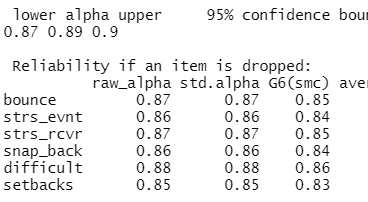
\includegraphics{images/resilience_reliability.png}
\end{frame}

\begin{frame}{Latent Variable 2 (Resilience): CFA}
\protect\hypertarget{latent-variable-2-resilience-cfa}{}
\centering

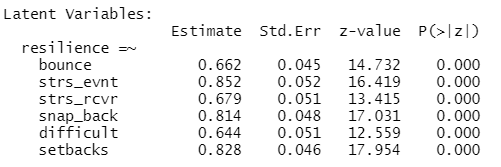
\includegraphics{images/resilience_cfa.png}

Fit statistics: CFI \textgreater{} 0.98, RMSEA \textless{} 0.08,
\(\chi^2\) = 0.017
\end{frame}

\begin{frame}[fragile]{Latent Variable 3: Healthy Lifestyle}
\protect\hypertarget{latent-variable-3-healthy-lifestyle}{}
We hypothesized that we could create a latent variable representing a
healthy lifestyle using the following variables:

\begin{itemize}
\item
  \texttt{fruit\_veg}: Five Fruit and Vegetables (Yes/No)
\item
  \texttt{smoking}: Smoking Status (7-point Likert scale)
\item
  \texttt{hr\_sleep}: Hour Sleep (numeric variable)
\end{itemize}
\end{frame}

\begin{frame}[fragile]{Latent Variable 3 (Healthy Lifestyle):
Reliability}
\protect\hypertarget{latent-variable-3-healthy-lifestyle-reliability}{}
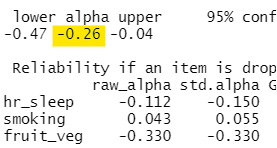
\includegraphics{images/health_alpha.png}

Chronbach's alpha is very low for these variables, indicating that the
variables \texttt{hr\_sleep}, \texttt{smoking}, \texttt{fruit\_veg} do
not reliably measure the latent variable.

Since \texttt{healthy\_lifestyle} is thus not reliably measured with
these variables, we made the decision to exclude this latent variable
from SEM analysis -- treating this latent variable as a formative
(rather than a reflective) construct might more accurately reflect its
nature.
\end{frame}

\begin{frame}{Outcome Variable: Mental Health Continuum Short Form
(MHC-SF)}
\protect\hypertarget{outcome-variable-mental-health-continuum-short-form-mhc-sf}{}
\centering

\begin{figure}
\centering
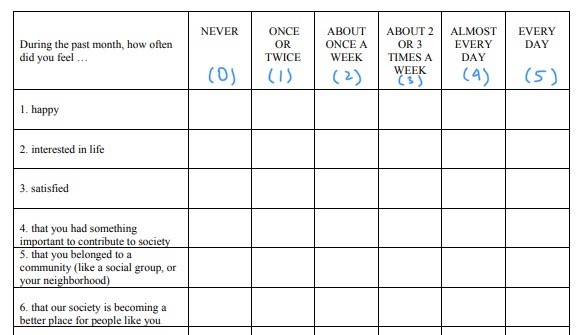
\includegraphics{images/mhc_sf.jpg}
\caption{Mental Health Continuum Short Form (MHC-SF)}
\end{figure}
\end{frame}

\begin{frame}{Outcome Variable: MHC-SF}
\protect\hypertarget{outcome-variable-mhc-sf}{}
Three components of well-being are assessed:

\begin{itemize}
\tightlist
\item
  Emotional
\item
  Social
\item
  Psychological
\end{itemize}

We will use the MHC-SF composite score (sum of all responses) as our
outcome variable. Higher scores indicate greater levels of positive
well-being.
\end{frame}

\begin{frame}{SEM 1: Athletic Identity and MHC-SF}
\protect\hypertarget{sem-1-athletic-identity-and-mhc-sf}{}
First, we constructed a SEM relating athletic identity to MHC-SF,
without any mediating variable.

\centering

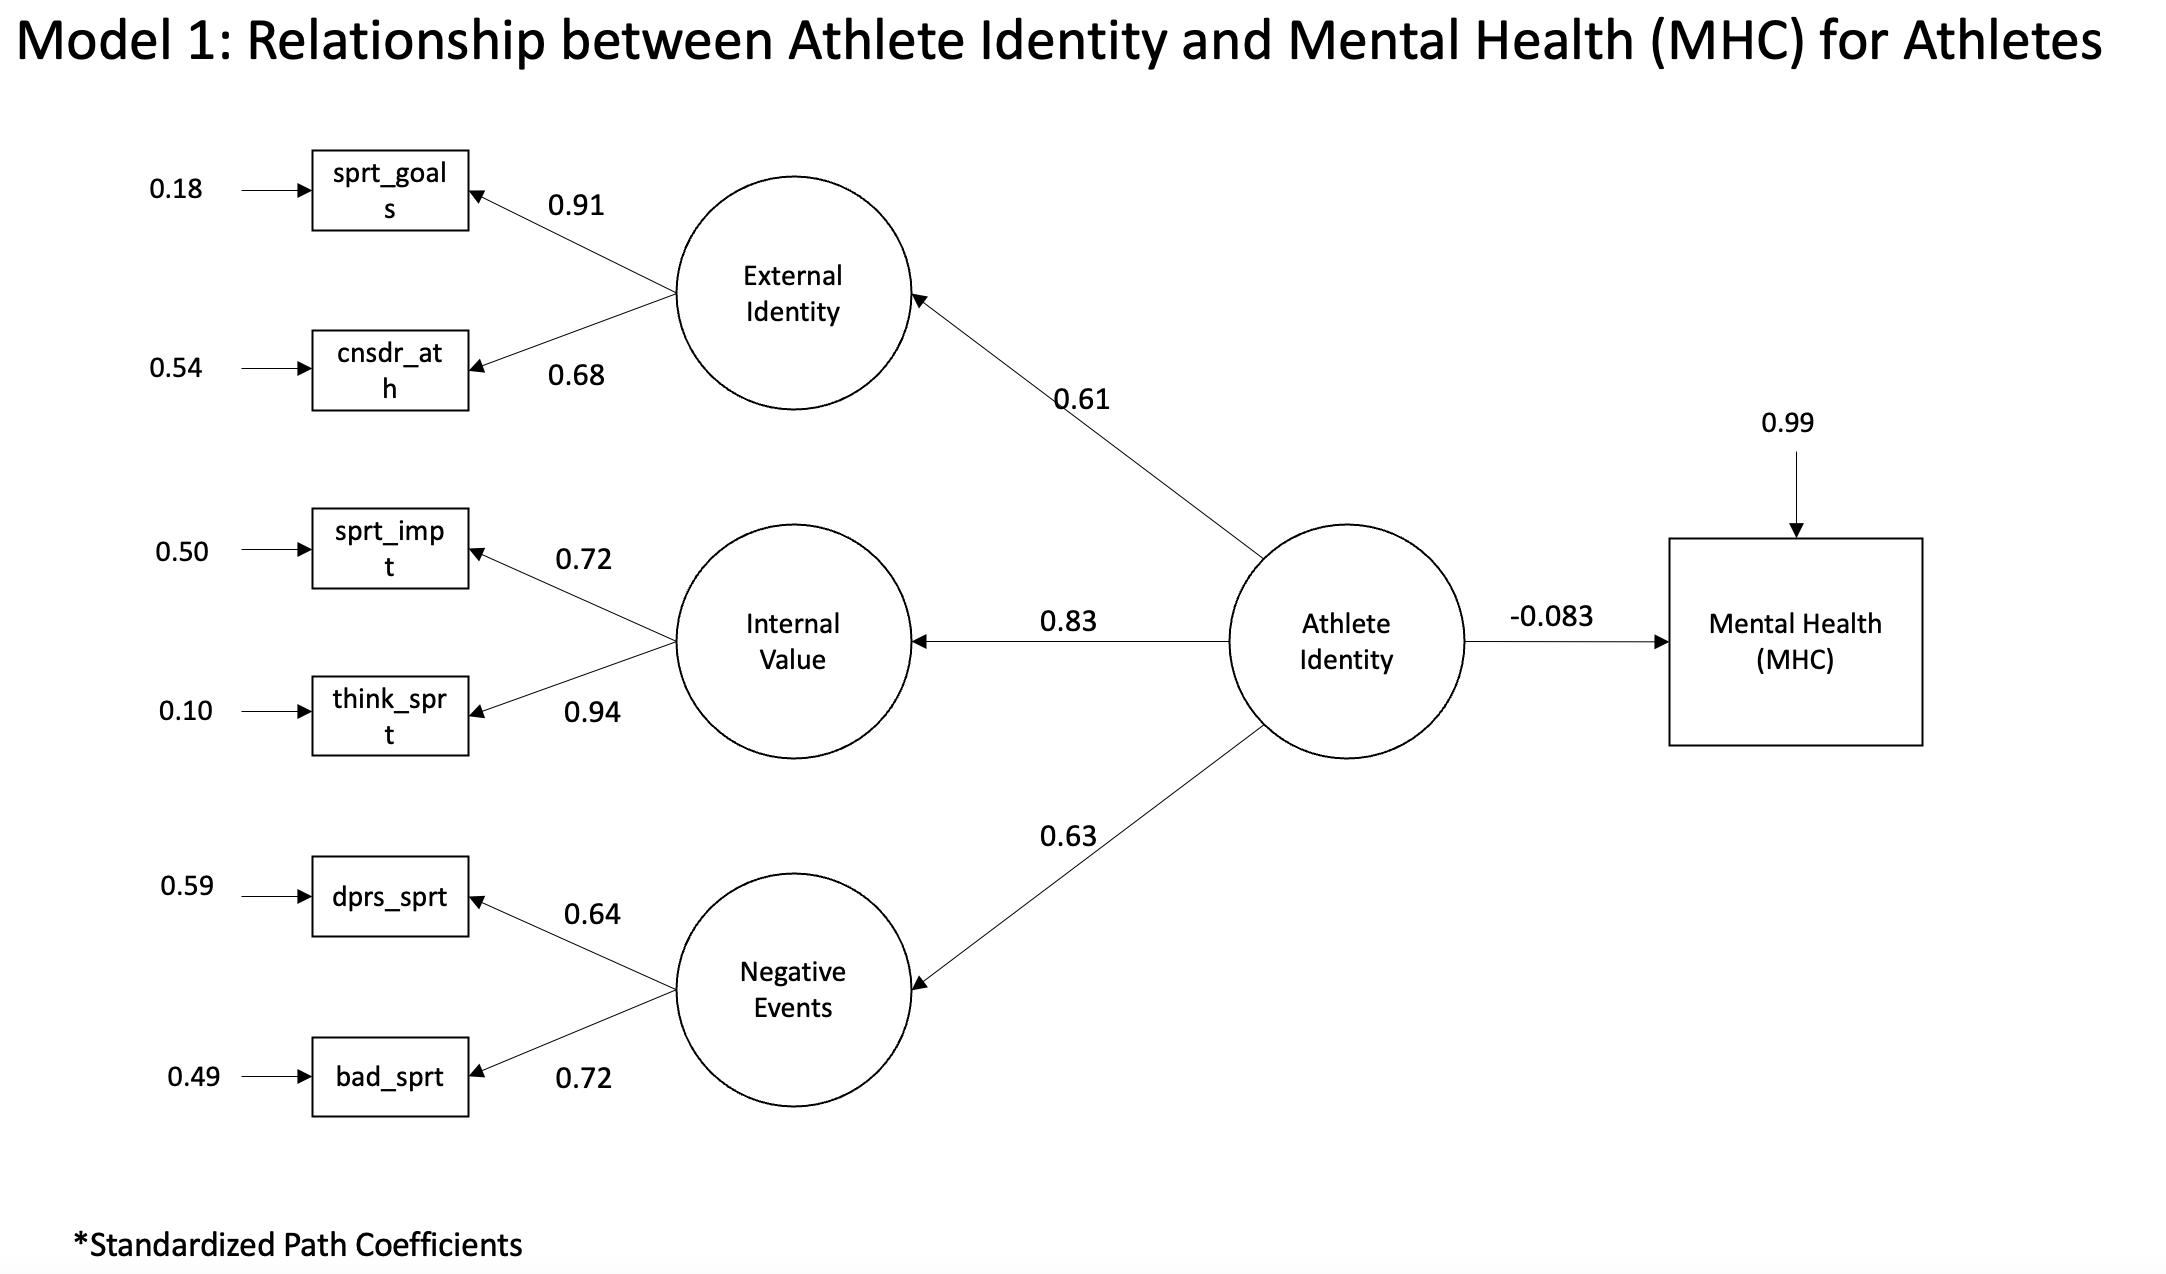
\includegraphics{images/SEM_1.png}
\end{frame}

\begin{frame}{SEM 1: Athletic Identity and MHC-SF}
\protect\hypertarget{sem-1-athletic-identity-and-mhc-sf-1}{}
We found that though the estimated effect between athletic identity and
MHC-SF is negative, indicating that a stronger athletic identity
decreases overall well-being, the p-value associated with this value is
0.232.

Therefore, we conclude that there is \textbf{no} significant
relationship between athletic identity and overall well-being.
\end{frame}

\begin{frame}{SEM 2: Resilience, Athletic Identity, and MHC-SF}
\protect\hypertarget{sem-2-resilience-athletic-identity-and-mhc-sf}{}
We constructed another SEM to investigate the mediation effect of
Resilience on causal relationship between athletic identity and MHC-SF.

\centering

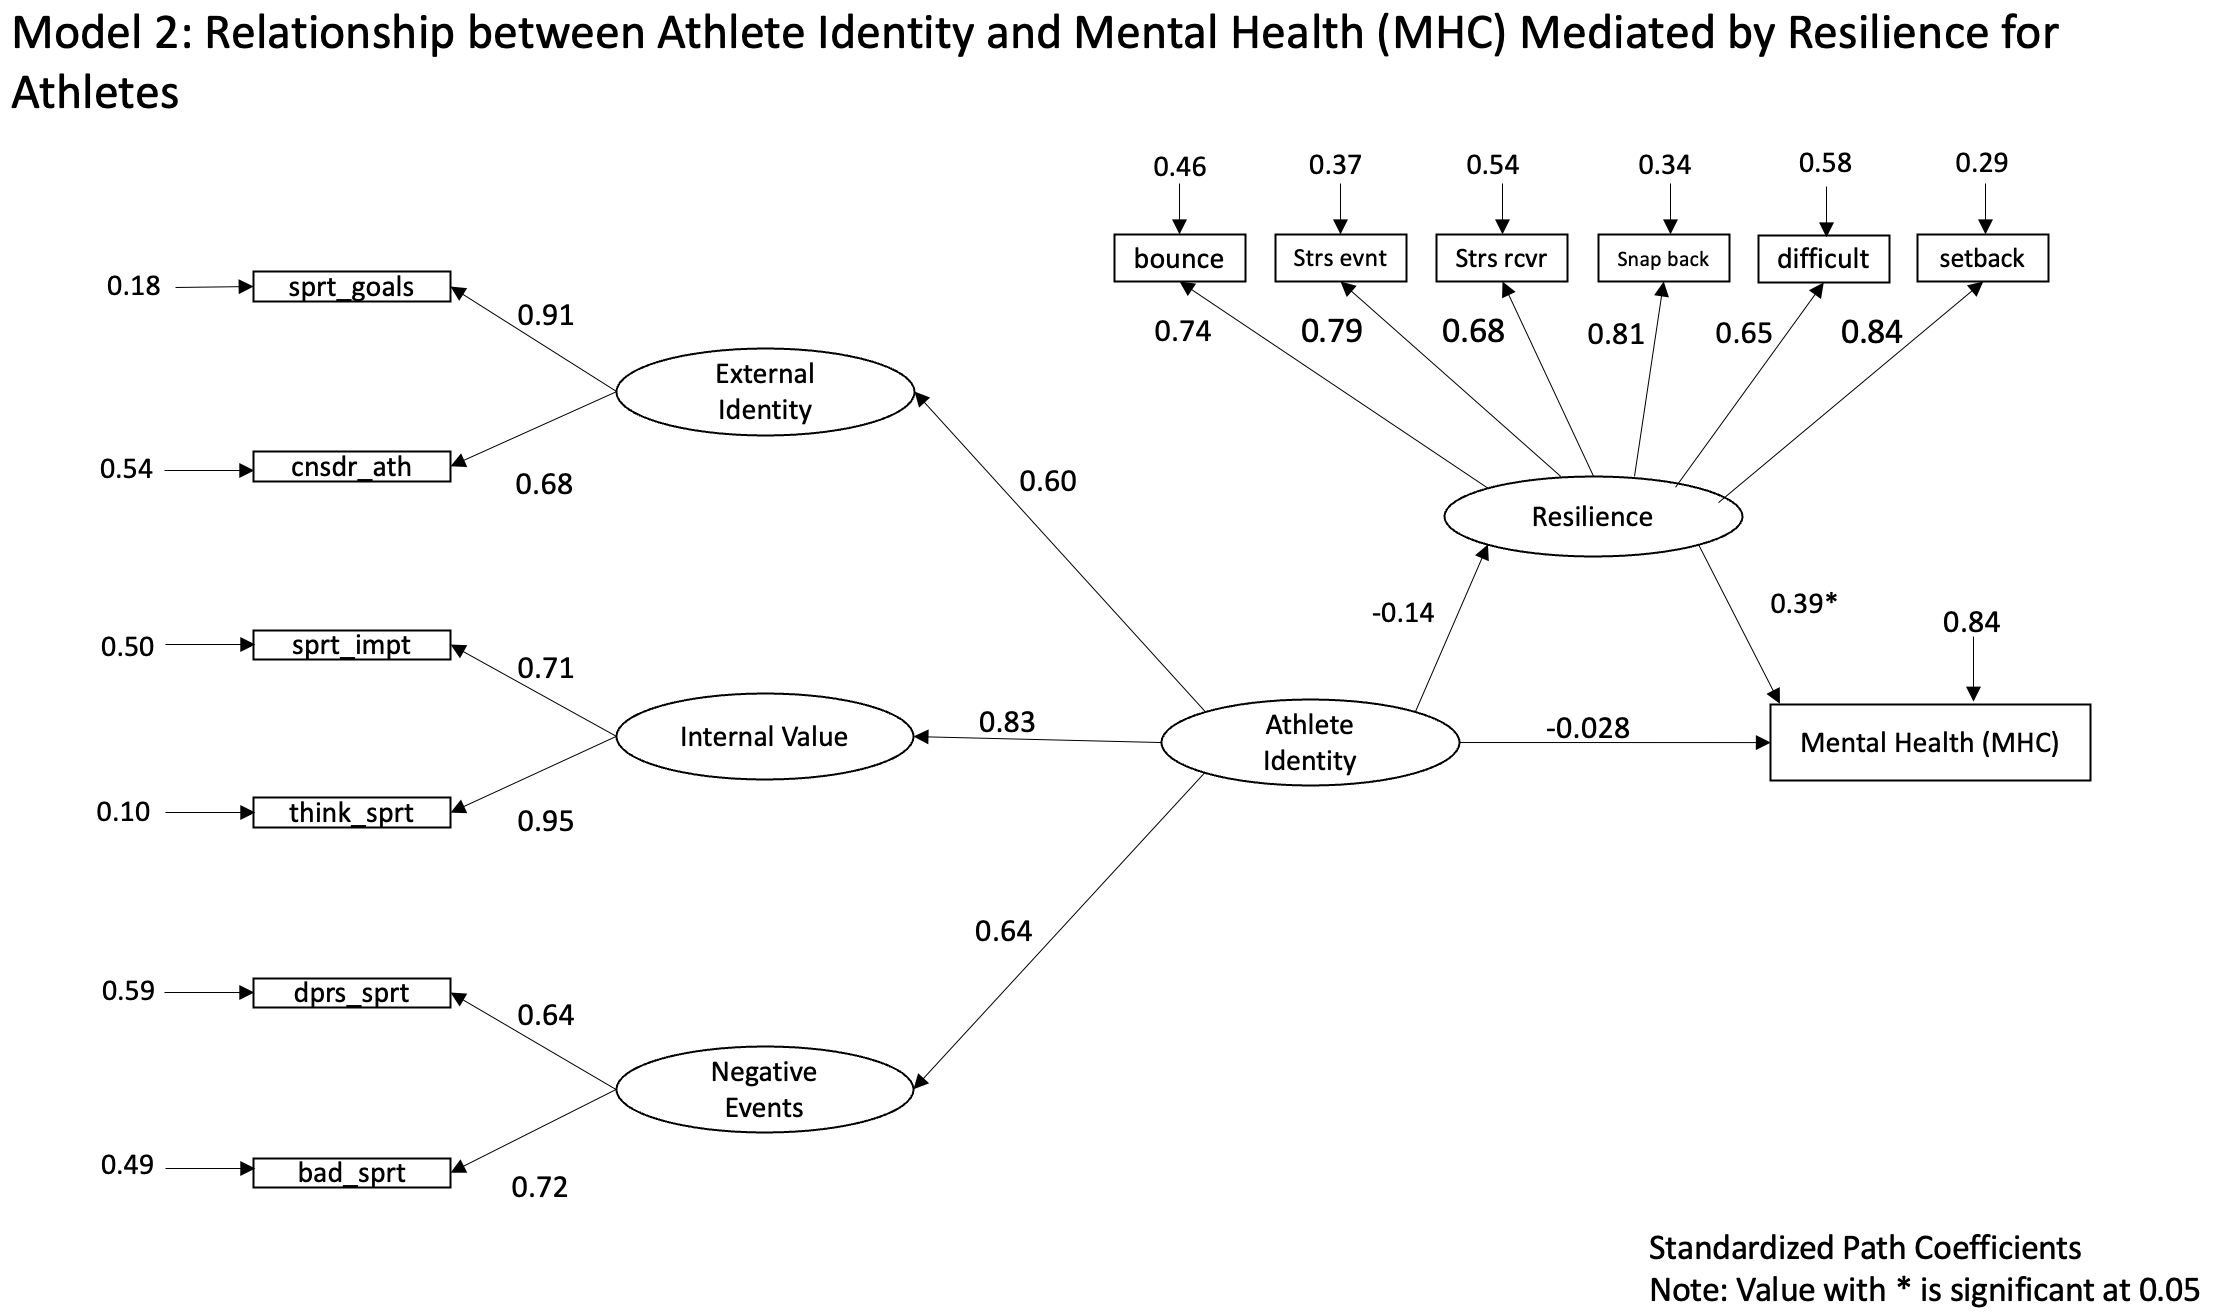
\includegraphics{images/SEM_2.png}
\end{frame}

\begin{frame}{SEM 2 : Conclusion}
\protect\hypertarget{sem-2-conclusion}{}
\end{frame}

\begin{frame}{SEM2: Resilience, Athletic Identity, and MHC-SF}
\protect\hypertarget{sem2-resilience-athletic-identity-and-mhc-sf}{}
We found that estimated effect between athletic identity and resilience
is negative, indicating that stronger athletic identity decreases
resilience. Such effect is not significant.

The estimated effect between resilience and MHC-SF is positive,
indicating that stronger resilience increases overall well-being. Such
effect is significant at 0.05 significant level.

\centering

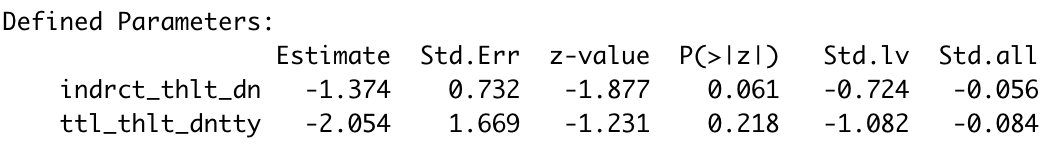
\includegraphics{images/standardized_direct_indirect.png}

\begin{itemize}
\tightlist
\item
  Both direct and indirect effects are not significant.
\end{itemize}
\end{frame}

\begin{frame}{Comparison of Athletes and Non-athletes}
\protect\hypertarget{comparison-of-athletes-and-non-athletes}{}
\begin{itemize}
\tightlist
\item
  We are interested in comparing mediation effects of resilience on
  relationship between athletic identity and MCH-SF within athlete group
  and non-athlete group
\end{itemize}

\centering

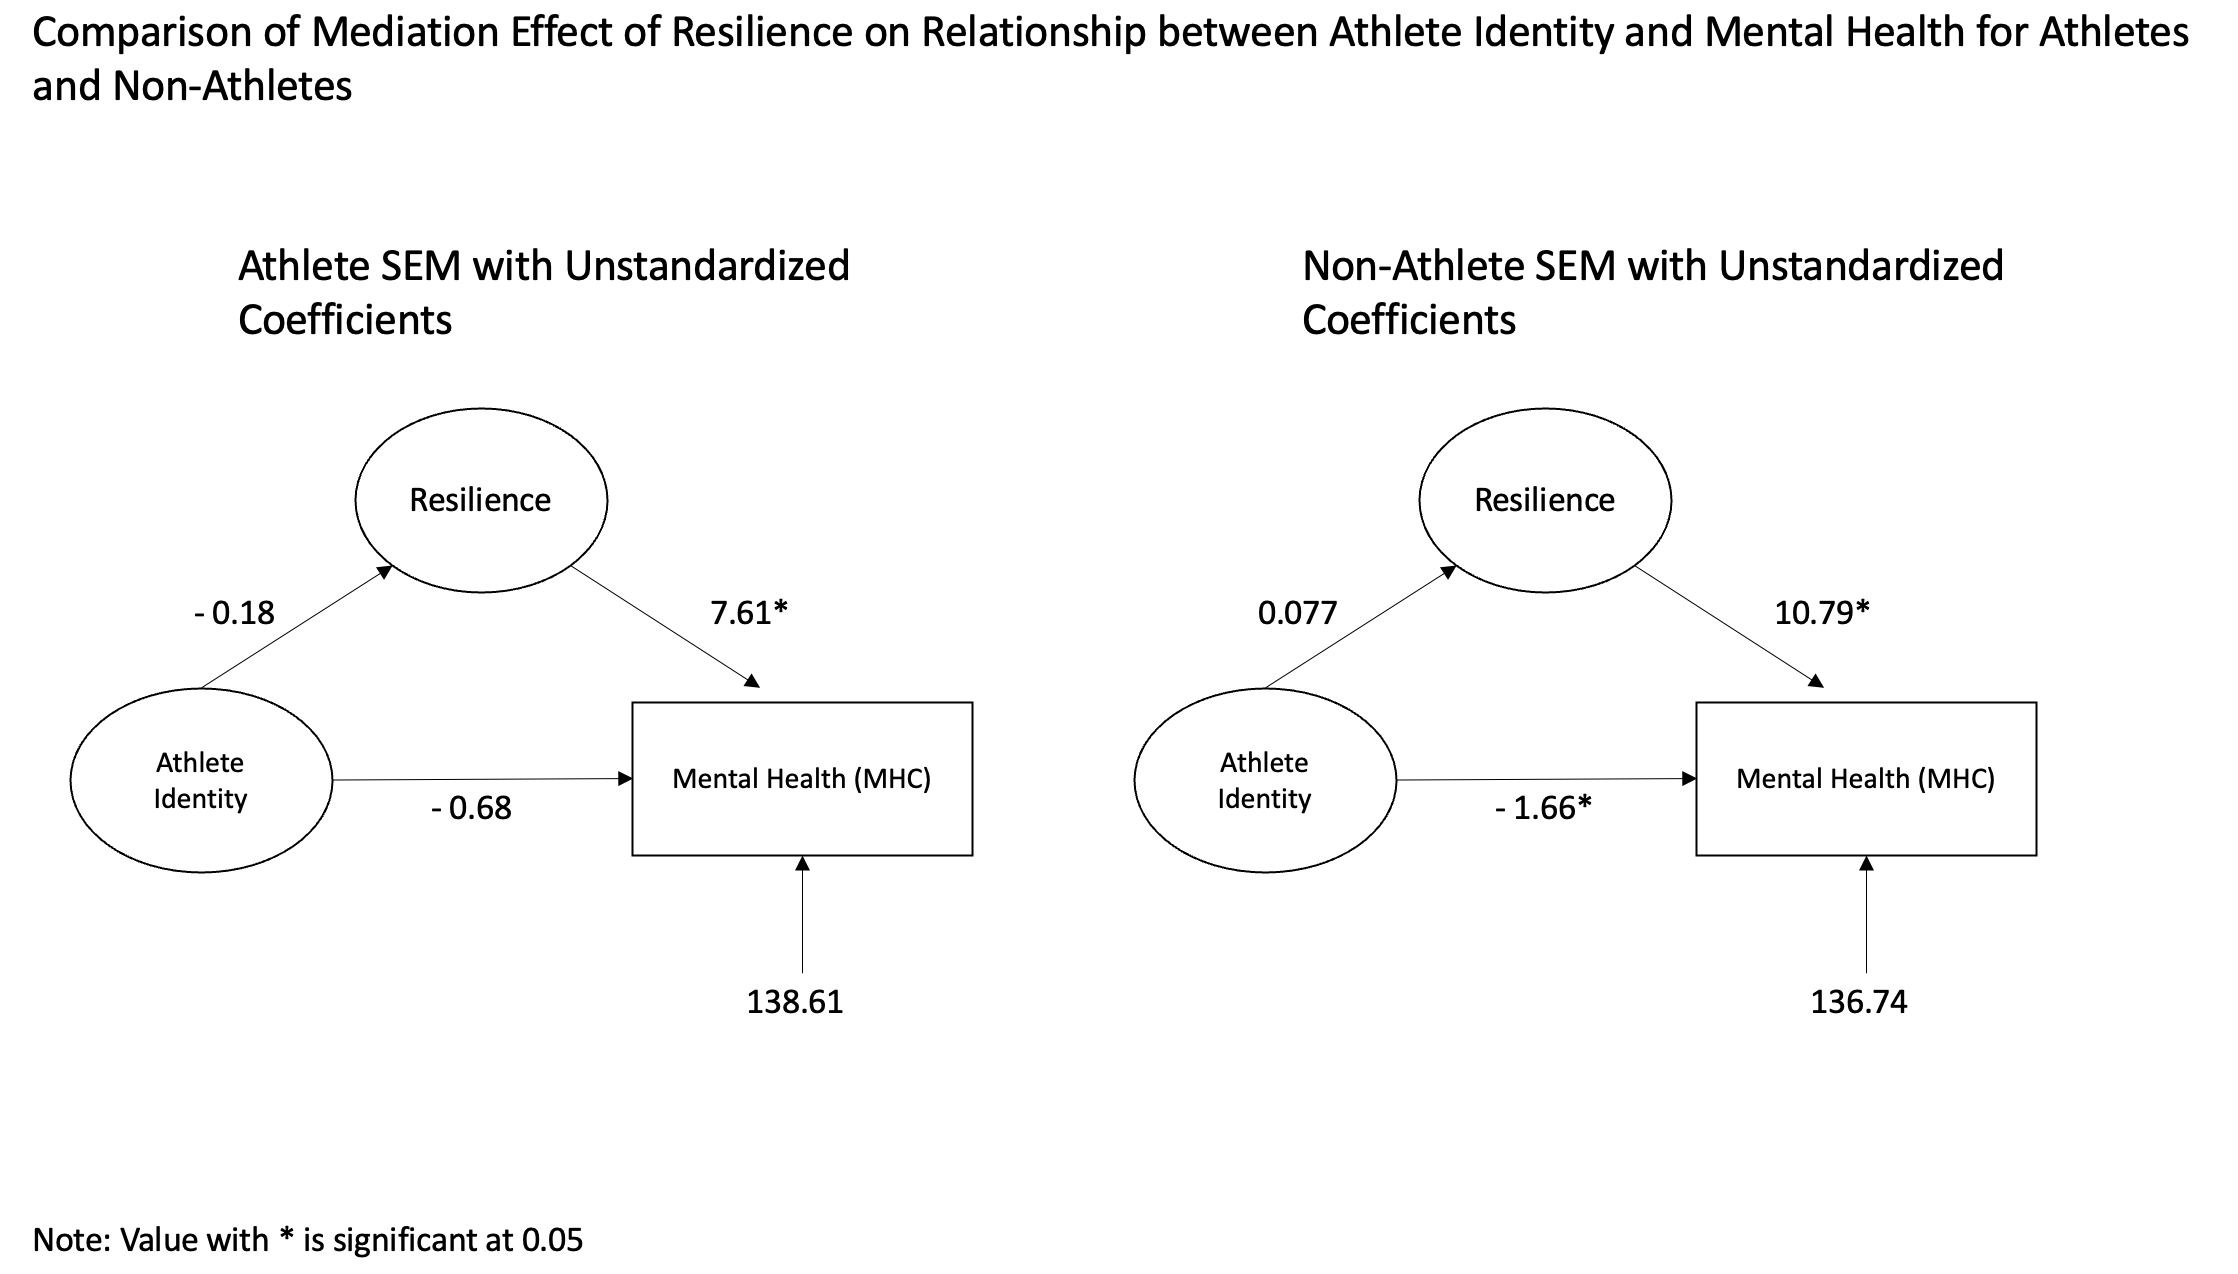
\includegraphics{images/SEM_3.png}
\end{frame}

\begin{frame}{Comparsion of SEM within Athletes and Non-athletes:
Conclusion}
\protect\hypertarget{comparsion-of-sem-within-athletes-and-non-athletes-conclusion}{}
\begin{itemize}
\item
  We found that the estimated effect between athletic identity and
  MHC-SF is stronger among non-athletes compared to athletes. Such
  effect is significant.
\item
  Direct/Indirect effect of athletic identity among athletes
  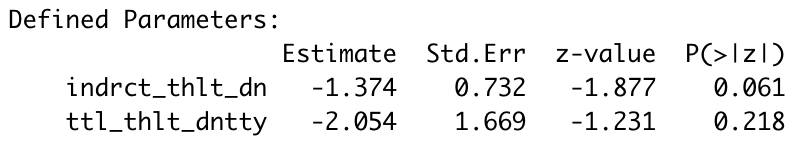
\includegraphics{images/athlete_unstandardized_direct_indirect.png}
\item
  Direct/Indirect effect of athletic identity among non-athletes
  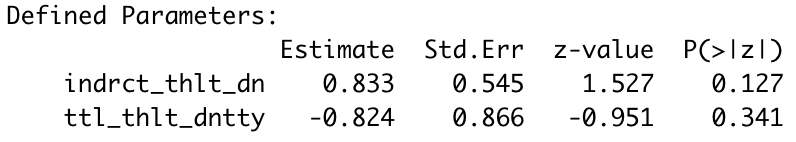
\includegraphics{images/non_athlete_unstandardized_direct_indirect.png}
\end{itemize}

\begin{quote}
\begin{quote}
\begin{quote}
\begin{quote}
\begin{quote}
\begin{quote}
\begin{quote}
ff3cd52c6319f990b80ad56c2587ceef5fd6632f
\end{quote}
\end{quote}
\end{quote}
\end{quote}
\end{quote}
\end{quote}
\end{quote}
\end{frame}

\begin{frame}{Resources}
\protect\hypertarget{resources}{}
\begin{enumerate}
\item
  Hu, T., Zhang, D., \& Wang, J. (2014, December 13). A meta-analysis of
  the Trait Resilience and Mental Health. Personality and Individual
  Differences.
  \url{https://www.sciencedirect.com/science/article/pii/S0191886914006710}
\item
  Dale, H., Brassington, L., \& King, K. (2014, March 5). The impact of
  healthy lifestyle interventions on Mental Health and Wellbeing: A
  systematic review. Mental Health Review Journal.
  \url{https://www.emerald.com/insight/content/doi/10.1108/MHRJ-05-2013-0016/full/html}
\item
  A cross-cultural psychometric evaluation of the Athletic Identity
  Measurement Scale. Taylor \& Francis. (n.d.).
  \url{https://www.tandfonline.com/doi/full/10.1080/10413200802415048}
\item
  The brief resilience scale. Evaluating wellbeing. (2021, March 15).
  \url{https://measure.whatworkswellbeing.org/measures-bank/brief-resilience-scale/}
\end{enumerate}
\end{frame}

\begin{frame}{Resources}
\protect\hypertarget{resources-1}{}
\begin{enumerate}
\setcounter{enumi}{4}
\item
  Fung S. F. (2020). Validity of the Brief Resilience Scale and Brief
  Resilient Coping Scale in a Chinese Sample. International journal of
  environmental research and public health, 17(4), 1265.
  \url{https://doi.org/10.3390/ijerph17041265}
\item
  Mental health continuum short form. Lee Kum Sheung Center for Health
  and Happiness. (2022, March 16). Retrieved May 3, 2022, from
  \url{https://www.hsph.harvard.edu/health-happiness/mental-health-continuum-short-form/}
\end{enumerate}
\end{frame}

\end{document}
